% Created by tikzDevice version 0.12.3 on 2020-12-22 01:51:45
% !TEX encoding = UTF-8 Unicode
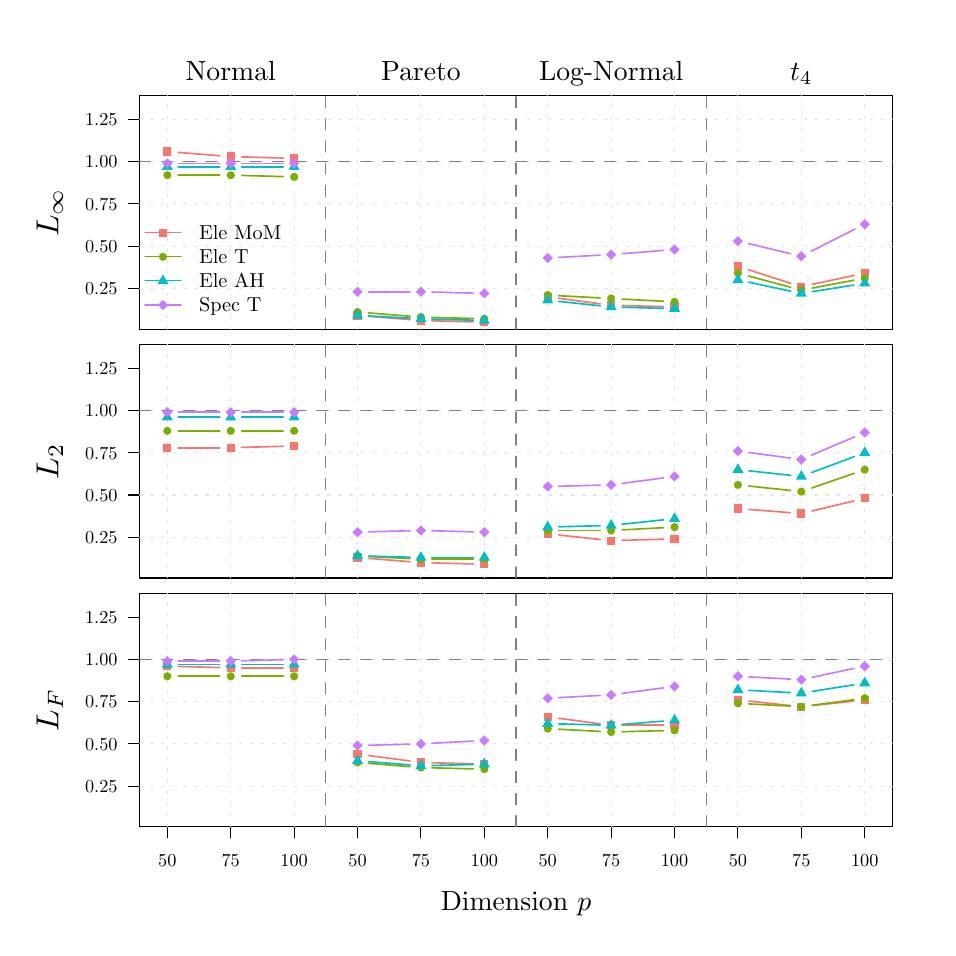
\begin{tikzpicture}[x=1pt,y=1pt]
\definecolor{fillColor}{RGB}{255,255,255}
\path[use as bounding box,fill=fillColor,fill opacity=0.00] (0,0) rectangle (325.21,325.21);
\begin{scope}
\path[clip] (  0.00,  0.00) rectangle (325.21,325.21);
\definecolor{drawColor}{RGB}{0,0,0}

\path[draw=drawColor,line width= 0.4pt,line join=round,line cap=round] ( 40.39,216.28) --
	(312.54,216.28) --
	(312.54,300.66) --
	( 40.39,300.66) --
	( 40.39,216.28);

\path[draw=drawColor,line width= 0.4pt,line join=round,line cap=round] ( 40.39,231.00) -- ( 40.39,292.04);

\path[draw=drawColor,line width= 0.4pt,line join=round,line cap=round] ( 40.39,231.00) -- ( 36.43,231.00);

\path[draw=drawColor,line width= 0.4pt,line join=round,line cap=round] ( 40.39,246.26) -- ( 36.43,246.26);

\path[draw=drawColor,line width= 0.4pt,line join=round,line cap=round] ( 40.39,261.52) -- ( 36.43,261.52);

\path[draw=drawColor,line width= 0.4pt,line join=round,line cap=round] ( 40.39,276.78) -- ( 36.43,276.78);

\path[draw=drawColor,line width= 0.4pt,line join=round,line cap=round] ( 40.39,292.04) -- ( 36.43,292.04);

\node[text=drawColor,anchor=base east,inner sep=0pt, outer sep=0pt, scale=  0.66] at ( 32.47,228.73) {0.25};

\node[text=drawColor,anchor=base east,inner sep=0pt, outer sep=0pt, scale=  0.66] at ( 32.47,243.99) {0.50};

\node[text=drawColor,anchor=base east,inner sep=0pt, outer sep=0pt, scale=  0.66] at ( 32.47,259.25) {0.75};

\node[text=drawColor,anchor=base east,inner sep=0pt, outer sep=0pt, scale=  0.66] at ( 32.47,274.51) {1.00};

\node[text=drawColor,anchor=base east,inner sep=0pt, outer sep=0pt, scale=  0.66] at ( 32.47,289.77) {1.25};
\end{scope}
\begin{scope}
\path[clip] ( 40.39,216.28) rectangle (312.54,300.66);
\definecolor{drawColor}{gray}{0.90}

\path[draw=drawColor,line width= 0.4pt,dash pattern=on 1pt off 3pt ,line join=round,line cap=round] ( 40.39,231.00) -- (312.54,231.00);

\path[draw=drawColor,line width= 0.4pt,dash pattern=on 1pt off 3pt ,line join=round,line cap=round] ( 40.39,246.26) -- (312.54,246.26);

\path[draw=drawColor,line width= 0.4pt,dash pattern=on 1pt off 3pt ,line join=round,line cap=round] ( 40.39,261.52) -- (312.54,261.52);

\path[draw=drawColor,line width= 0.4pt,dash pattern=on 1pt off 3pt ,line join=round,line cap=round] ( 40.39,276.78) -- (312.54,276.78);

\path[draw=drawColor,line width= 0.4pt,dash pattern=on 1pt off 3pt ,line join=round,line cap=round] ( 40.39,292.04) -- (312.54,292.04);

\path[draw=drawColor,line width= 0.4pt,dash pattern=on 1pt off 3pt ,line join=round,line cap=round] ( 50.47,216.28) -- ( 50.47,300.66);

\path[draw=drawColor,line width= 0.4pt,dash pattern=on 1pt off 3pt ,line join=round,line cap=round] ( 73.38,216.28) -- ( 73.38,300.66);

\path[draw=drawColor,line width= 0.4pt,dash pattern=on 1pt off 3pt ,line join=round,line cap=round] ( 96.29,216.28) -- ( 96.29,300.66);

\path[draw=drawColor,line width= 0.4pt,dash pattern=on 1pt off 3pt ,line join=round,line cap=round] (119.20,216.28) -- (119.20,300.66);

\path[draw=drawColor,line width= 0.4pt,dash pattern=on 1pt off 3pt ,line join=round,line cap=round] (142.10,216.28) -- (142.10,300.66);

\path[draw=drawColor,line width= 0.4pt,dash pattern=on 1pt off 3pt ,line join=round,line cap=round] (165.01,216.28) -- (165.01,300.66);

\path[draw=drawColor,line width= 0.4pt,dash pattern=on 1pt off 3pt ,line join=round,line cap=round] (187.92,216.28) -- (187.92,300.66);

\path[draw=drawColor,line width= 0.4pt,dash pattern=on 1pt off 3pt ,line join=round,line cap=round] (210.83,216.28) -- (210.83,300.66);

\path[draw=drawColor,line width= 0.4pt,dash pattern=on 1pt off 3pt ,line join=round,line cap=round] (233.74,216.28) -- (233.74,300.66);

\path[draw=drawColor,line width= 0.4pt,dash pattern=on 1pt off 3pt ,line join=round,line cap=round] (256.65,216.28) -- (256.65,300.66);

\path[draw=drawColor,line width= 0.4pt,dash pattern=on 1pt off 3pt ,line join=round,line cap=round] (279.56,216.28) -- (279.56,300.66);

\path[draw=drawColor,line width= 0.4pt,dash pattern=on 1pt off 3pt ,line join=round,line cap=round] (302.46,216.28) -- (302.46,300.66);
\definecolor{drawColor}{gray}{0.50}

\path[draw=drawColor,line width= 0.4pt,dash pattern=on 4pt off 4pt ,line join=round,line cap=round] (107.74,216.28) -- (107.74,300.66);

\path[draw=drawColor,line width= 0.4pt,dash pattern=on 4pt off 4pt ,line join=round,line cap=round] (176.47,216.28) -- (176.47,300.66);

\path[draw=drawColor,line width= 0.4pt,dash pattern=on 4pt off 4pt ,line join=round,line cap=round] (245.19,216.28) -- (245.19,300.66);

\path[draw=drawColor,line width= 0.4pt,dash pattern=on 4pt off 4pt ,line join=round,line cap=round] (313.92,216.28) -- (313.92,300.66);
\end{scope}
\begin{scope}
\path[clip] (  0.00,  0.00) rectangle (325.21,325.21);
\definecolor{drawColor}{RGB}{0,0,0}

\node[text=drawColor,rotate= 90.00,anchor=base,inner sep=0pt, outer sep=0pt, scale=  1.15] at ( 11.09,258.47) {$L_{\infty}$};
\end{scope}
\begin{scope}
\path[clip] ( 40.39,216.28) rectangle (312.54,300.66);
\definecolor{drawColor}{gray}{0.50}

\path[draw=drawColor,line width= 0.4pt,dash pattern=on 4pt off 4pt ,line join=round,line cap=round] ( 40.39,276.78) -- (312.54,276.78);
\end{scope}
\begin{scope}
\path[clip] (  0.00,  0.00) rectangle (325.21,325.21);
\definecolor{drawColor}{RGB}{0,0,0}

\node[text=drawColor,anchor=base,inner sep=0pt, outer sep=0pt, scale=  1.00] at ( 73.38,306.21) {Normal};

\node[text=drawColor,anchor=base,inner sep=0pt, outer sep=0pt, scale=  1.00] at (142.10,306.21) {Pareto};

\node[text=drawColor,anchor=base,inner sep=0pt, outer sep=0pt, scale=  1.00] at (210.83,306.21) {Log-Normal};

\node[text=drawColor,anchor=base,inner sep=0pt, outer sep=0pt, scale=  1.00] at (279.56,306.21) {$t_4$};
\end{scope}
\begin{scope}
\path[clip] ( 40.39,216.28) rectangle (312.54,300.66);
\definecolor{drawColor}{RGB}{248,118,109}

\path[draw=drawColor,line width= 0.4pt,line join=round,line cap=round] ( 42.35,251.13) -- ( 55.42,251.13);
\definecolor{drawColor}{RGB}{124,174,0}

\path[draw=drawColor,line width= 0.4pt,line join=round,line cap=round] ( 42.35,242.42) -- ( 55.42,242.42);
\definecolor{drawColor}{RGB}{0,191,196}

\path[draw=drawColor,line width= 0.4pt,line join=round,line cap=round] ( 42.35,233.71) -- ( 55.42,233.71);
\definecolor{drawColor}{RGB}{199,124,255}

\path[draw=drawColor,line width= 0.4pt,line join=round,line cap=round] ( 42.35,224.99) -- ( 55.42,224.99);
\definecolor{fillColor}{RGB}{248,118,109}

\path[fill=fillColor] ( 47.40,249.64) --
	( 50.37,249.64) --
	( 50.37,252.61) --
	( 47.40,252.61) --
	cycle;
\definecolor{fillColor}{RGB}{124,174,0}

\path[fill=fillColor] ( 48.89,242.42) circle (  1.48);
\definecolor{fillColor}{RGB}{0,191,196}

\path[fill=fillColor] ( 48.89,236.02) --
	( 50.89,232.55) --
	( 46.89,232.55) --
	cycle;
\definecolor{fillColor}{RGB}{199,124,255}

\path[fill=fillColor] ( 47.03,224.99) --
	( 48.89,226.85) --
	( 50.74,224.99) --
	( 48.89,223.14) --
	cycle;
\definecolor{drawColor}{RGB}{0,0,0}

\node[text=drawColor,anchor=base west,inner sep=0pt, outer sep=0pt, scale=  0.73] at ( 61.95,248.63) {Ele MoM};

\node[text=drawColor,anchor=base west,inner sep=0pt, outer sep=0pt, scale=  0.73] at ( 61.95,239.92) {Ele T};

\node[text=drawColor,anchor=base west,inner sep=0pt, outer sep=0pt, scale=  0.73] at ( 61.95,231.21) {Ele AH};

\node[text=drawColor,anchor=base west,inner sep=0pt, outer sep=0pt, scale=  0.73] at ( 61.95,222.49) {Spec T};
\definecolor{drawColor}{RGB}{248,118,109}

\path[draw=drawColor,line width= 0.6pt,line join=round,line cap=round] ( 54.42,280.13) -- ( 69.43,278.93);

\path[draw=drawColor,line width= 0.6pt,line join=round,line cap=round] ( 77.34,278.51) -- ( 92.33,278.11);
\definecolor{fillColor}{RGB}{248,118,109}

\path[fill=fillColor] ( 48.99,278.96) --
	( 51.96,278.96) --
	( 51.96,281.93) --
	( 48.99,281.93) --
	cycle;

\path[fill=fillColor] ( 71.89,277.13) --
	( 74.86,277.13) --
	( 74.86,280.10) --
	( 71.89,280.10) --
	cycle;

\path[fill=fillColor] ( 94.80,276.52) --
	( 97.77,276.52) --
	( 97.77,279.49) --
	( 94.80,279.49) --
	cycle;
\definecolor{drawColor}{RGB}{124,174,0}

\path[draw=drawColor,line width= 0.6pt,line join=round,line cap=round] ( 54.43,271.90) -- ( 69.42,271.90);

\path[draw=drawColor,line width= 0.6pt,line join=round,line cap=round] ( 77.34,271.80) -- ( 92.33,271.40);
\definecolor{fillColor}{RGB}{124,174,0}

\path[fill=fillColor] ( 50.47,271.90) circle (  1.48);

\path[fill=fillColor] ( 73.38,271.90) circle (  1.48);

\path[fill=fillColor] ( 96.29,271.29) circle (  1.48);
\definecolor{drawColor}{RGB}{0,191,196}

\path[draw=drawColor,line width= 0.6pt,line join=round,line cap=round] ( 54.43,274.95) -- ( 69.42,274.95);

\path[draw=drawColor,line width= 0.6pt,line join=round,line cap=round] ( 77.34,274.95) -- ( 92.33,274.95);
\definecolor{fillColor}{RGB}{0,191,196}

\path[fill=fillColor] ( 50.47,277.26) --
	( 52.47,273.80) --
	( 48.47,273.80) --
	cycle;

\path[fill=fillColor] ( 73.38,277.26) --
	( 75.38,273.80) --
	( 71.38,273.80) --
	cycle;

\path[fill=fillColor] ( 96.29,277.26) --
	( 98.29,273.80) --
	( 94.29,273.80) --
	cycle;
\definecolor{drawColor}{RGB}{199,124,255}

\path[draw=drawColor,line width= 0.6pt,line join=round,line cap=round] ( 54.43,276.17) -- ( 69.42,276.17);

\path[draw=drawColor,line width= 0.6pt,line join=round,line cap=round] ( 77.34,276.17) -- ( 92.33,276.17);
\definecolor{fillColor}{RGB}{199,124,255}

\path[fill=fillColor] ( 48.62,276.17) --
	( 50.47,278.03) --
	( 52.33,276.17) --
	( 50.47,274.32) --
	cycle;

\path[fill=fillColor] ( 71.52,276.17) --
	( 73.38,278.03) --
	( 75.24,276.17) --
	( 73.38,274.32) --
	cycle;

\path[fill=fillColor] ( 94.43,276.17) --
	( 96.29,278.03) --
	( 98.14,276.17) --
	( 96.29,274.32) --
	cycle;
\definecolor{drawColor}{RGB}{248,118,109}

\path[draw=drawColor,line width= 0.6pt,line join=round,line cap=round] (123.14,220.92) -- (138.16,219.72);

\path[draw=drawColor,line width= 0.6pt,line join=round,line cap=round] (146.06,219.30) -- (161.05,218.90);
\definecolor{fillColor}{RGB}{248,118,109}

\path[fill=fillColor] (117.71,219.75) --
	(120.68,219.75) --
	(120.68,222.72) --
	(117.71,222.72) --
	cycle;

\path[fill=fillColor] (140.62,217.92) --
	(143.59,217.92) --
	(143.59,220.89) --
	(140.62,220.89) --
	cycle;

\path[fill=fillColor] (163.53,217.31) --
	(166.50,217.31) --
	(166.50,220.28) --
	(163.53,220.28) --
	cycle;
\definecolor{drawColor}{RGB}{124,174,0}

\path[draw=drawColor,line width= 0.6pt,line join=round,line cap=round] (123.14,222.14) -- (138.16,220.94);

\path[draw=drawColor,line width= 0.6pt,line join=round,line cap=round] (146.06,220.52) -- (161.05,220.12);
\definecolor{fillColor}{RGB}{124,174,0}

\path[fill=fillColor] (119.20,222.46) circle (  1.48);

\path[fill=fillColor] (142.10,220.63) circle (  1.48);

\path[fill=fillColor] (165.01,220.02) circle (  1.48);
\definecolor{drawColor}{RGB}{0,191,196}

\path[draw=drawColor,line width= 0.6pt,line join=round,line cap=round] (123.15,221.03) -- (138.15,220.23);

\path[draw=drawColor,line width= 0.6pt,line join=round,line cap=round] (146.06,219.91) -- (161.05,219.51);
\definecolor{fillColor}{RGB}{0,191,196}

\path[fill=fillColor] (119.20,223.55) --
	(121.20,220.08) --
	(117.20,220.08) --
	cycle;

\path[fill=fillColor] (142.10,222.33) --
	(144.10,218.86) --
	(140.11,218.86) --
	cycle;

\path[fill=fillColor] (165.01,221.72) --
	(167.01,218.25) --
	(163.01,218.25) --
	cycle;
\definecolor{drawColor}{RGB}{199,124,255}

\path[draw=drawColor,line width= 0.6pt,line join=round,line cap=round] (123.16,229.78) -- (138.14,229.78);

\path[draw=drawColor,line width= 0.6pt,line join=round,line cap=round] (146.06,229.68) -- (161.05,229.28);
\definecolor{fillColor}{RGB}{199,124,255}

\path[fill=fillColor] (117.34,229.78) --
	(119.20,231.64) --
	(121.05,229.78) --
	(119.20,227.93) --
	cycle;

\path[fill=fillColor] (140.25,229.78) --
	(142.10,231.64) --
	(143.96,229.78) --
	(142.10,227.93) --
	cycle;

\path[fill=fillColor] (163.16,229.17) --
	(165.01,231.03) --
	(166.87,229.17) --
	(165.01,227.32) --
	cycle;
\definecolor{drawColor}{RGB}{248,118,109}

\path[draw=drawColor,line width= 0.6pt,line join=round,line cap=round] (191.85,227.43) -- (206.90,225.42);

\path[draw=drawColor,line width= 0.6pt,line join=round,line cap=round] (214.79,224.80) -- (229.78,224.40);
\definecolor{fillColor}{RGB}{248,118,109}

\path[fill=fillColor] (186.44,226.47) --
	(189.41,226.47) --
	(189.41,229.44) --
	(186.44,229.44) --
	cycle;

\path[fill=fillColor] (209.34,223.42) --
	(212.31,223.42) --
	(212.31,226.39) --
	(209.34,226.39) --
	cycle;

\path[fill=fillColor] (232.25,222.81) --
	(235.22,222.81) --
	(235.22,225.78) --
	(232.25,225.78) --
	cycle;
\definecolor{drawColor}{RGB}{124,174,0}

\path[draw=drawColor,line width= 0.6pt,line join=round,line cap=round] (191.88,228.35) -- (206.88,227.55);

\path[draw=drawColor,line width= 0.6pt,line join=round,line cap=round] (214.78,227.13) -- (229.78,226.33);
\definecolor{fillColor}{RGB}{124,174,0}

\path[fill=fillColor] (187.92,228.56) circle (  1.48);

\path[fill=fillColor] (210.83,227.34) circle (  1.48);

\path[fill=fillColor] (233.74,226.12) circle (  1.48);
\definecolor{drawColor}{RGB}{0,191,196}

\path[draw=drawColor,line width= 0.6pt,line join=round,line cap=round] (191.86,226.31) -- (206.89,224.71);

\path[draw=drawColor,line width= 0.6pt,line join=round,line cap=round] (214.79,224.18) -- (229.78,223.79);
\definecolor{fillColor}{RGB}{0,191,196}

\path[fill=fillColor] (187.92,229.04) --
	(189.92,225.58) --
	(185.92,225.58) --
	cycle;

\path[fill=fillColor] (210.83,226.60) --
	(212.83,223.14) --
	(208.83,223.14) --
	cycle;

\path[fill=fillColor] (233.74,225.99) --
	(235.74,222.53) --
	(231.74,222.53) --
	cycle;
\definecolor{drawColor}{RGB}{199,124,255}

\path[draw=drawColor,line width= 0.6pt,line join=round,line cap=round] (191.88,242.20) -- (206.88,243.00);

\path[draw=drawColor,line width= 0.6pt,line join=round,line cap=round] (214.78,243.53) -- (229.79,244.73);
\definecolor{fillColor}{RGB}{199,124,255}

\path[fill=fillColor] (186.07,241.99) --
	(187.92,243.85) --
	(189.78,241.99) --
	(187.92,240.14) --
	cycle;

\path[fill=fillColor] (208.97,243.21) --
	(210.83,245.07) --
	(212.69,243.21) --
	(210.83,241.36) --
	cycle;

\path[fill=fillColor] (231.88,245.04) --
	(233.74,246.90) --
	(235.59,245.04) --
	(233.74,243.19) --
	cycle;
\definecolor{drawColor}{RGB}{248,118,109}

\path[draw=drawColor,line width= 0.6pt,line join=round,line cap=round] (260.42,237.73) -- (275.78,232.82);

\path[draw=drawColor,line width= 0.6pt,line join=round,line cap=round] (283.43,232.44) -- (298.59,235.67);
\definecolor{fillColor}{RGB}{248,118,109}

\path[fill=fillColor] (255.16,237.45) --
	(258.13,237.45) --
	(258.13,240.42) --
	(255.16,240.42) --
	cycle;

\path[fill=fillColor] (278.07,230.13) --
	(281.04,230.13) --
	(281.04,233.10) --
	(278.07,233.10) --
	cycle;

\path[fill=fillColor] (300.98,235.01) --
	(303.95,235.01) --
	(303.95,237.98) --
	(300.98,237.98) --
	cycle;
\definecolor{drawColor}{RGB}{124,174,0}

\path[draw=drawColor,line width= 0.6pt,line join=round,line cap=round] (260.47,235.48) -- (275.73,231.41);

\path[draw=drawColor,line width= 0.6pt,line join=round,line cap=round] (283.45,231.12) -- (298.57,233.94);
\definecolor{fillColor}{RGB}{124,174,0}

\path[fill=fillColor] (256.65,236.50) circle (  1.48);

\path[fill=fillColor] (279.56,230.39) circle (  1.48);

\path[fill=fillColor] (302.46,234.67) circle (  1.48);
\definecolor{drawColor}{RGB}{0,191,196}

\path[draw=drawColor,line width= 0.6pt,line join=round,line cap=round] (260.52,233.23) -- (275.68,230.00);

\path[draw=drawColor,line width= 0.6pt,line join=round,line cap=round] (283.47,229.80) -- (298.55,232.21);
\definecolor{fillColor}{RGB}{0,191,196}

\path[fill=fillColor] (256.65,236.37) --
	(258.65,232.90) --
	(254.65,232.90) --
	cycle;

\path[fill=fillColor] (279.56,231.48) --
	(281.55,228.02) --
	(277.56,228.02) --
	cycle;

\path[fill=fillColor] (302.46,235.15) --
	(304.46,231.68) --
	(300.46,231.68) --
	cycle;
\definecolor{drawColor}{RGB}{199,124,255}

\path[draw=drawColor,line width= 0.6pt,line join=round,line cap=round] (260.50,247.17) -- (275.70,243.53);

\path[draw=drawColor,line width= 0.6pt,line join=round,line cap=round] (283.09,244.39) -- (298.93,252.41);
\definecolor{fillColor}{RGB}{199,124,255}

\path[fill=fillColor] (254.79,248.10) --
	(256.65,249.95) --
	(258.50,248.10) --
	(256.65,246.24) --
	cycle;

\path[fill=fillColor] (277.70,242.60) --
	(279.56,244.46) --
	(281.41,242.60) --
	(279.56,240.75) --
	cycle;

\path[fill=fillColor] (300.61,254.20) --
	(302.46,256.06) --
	(304.32,254.20) --
	(302.46,252.34) --
	cycle;
\end{scope}
\begin{scope}
\path[clip] (  0.00,  0.00) rectangle (325.21,325.21);
\definecolor{drawColor}{RGB}{0,0,0}

\path[draw=drawColor,line width= 0.4pt,line join=round,line cap=round] ( 40.39,126.36) --
	(312.54,126.36) --
	(312.54,210.74) --
	( 40.39,210.74) --
	( 40.39,126.36);

\path[draw=drawColor,line width= 0.4pt,line join=round,line cap=round] ( 40.39,141.08) -- ( 40.39,202.12);

\path[draw=drawColor,line width= 0.4pt,line join=round,line cap=round] ( 40.39,141.08) -- ( 36.43,141.08);

\path[draw=drawColor,line width= 0.4pt,line join=round,line cap=round] ( 40.39,156.34) -- ( 36.43,156.34);

\path[draw=drawColor,line width= 0.4pt,line join=round,line cap=round] ( 40.39,171.60) -- ( 36.43,171.60);

\path[draw=drawColor,line width= 0.4pt,line join=round,line cap=round] ( 40.39,186.86) -- ( 36.43,186.86);

\path[draw=drawColor,line width= 0.4pt,line join=round,line cap=round] ( 40.39,202.12) -- ( 36.43,202.12);

\node[text=drawColor,anchor=base east,inner sep=0pt, outer sep=0pt, scale=  0.66] at ( 32.47,138.81) {0.25};

\node[text=drawColor,anchor=base east,inner sep=0pt, outer sep=0pt, scale=  0.66] at ( 32.47,154.07) {0.50};

\node[text=drawColor,anchor=base east,inner sep=0pt, outer sep=0pt, scale=  0.66] at ( 32.47,169.33) {0.75};

\node[text=drawColor,anchor=base east,inner sep=0pt, outer sep=0pt, scale=  0.66] at ( 32.47,184.59) {1.00};

\node[text=drawColor,anchor=base east,inner sep=0pt, outer sep=0pt, scale=  0.66] at ( 32.47,199.85) {1.25};
\end{scope}
\begin{scope}
\path[clip] ( 40.39,126.36) rectangle (312.54,210.74);
\definecolor{drawColor}{gray}{0.90}

\path[draw=drawColor,line width= 0.4pt,dash pattern=on 1pt off 3pt ,line join=round,line cap=round] ( 40.39,141.08) -- (312.54,141.08);

\path[draw=drawColor,line width= 0.4pt,dash pattern=on 1pt off 3pt ,line join=round,line cap=round] ( 40.39,156.34) -- (312.54,156.34);

\path[draw=drawColor,line width= 0.4pt,dash pattern=on 1pt off 3pt ,line join=round,line cap=round] ( 40.39,171.60) -- (312.54,171.60);

\path[draw=drawColor,line width= 0.4pt,dash pattern=on 1pt off 3pt ,line join=round,line cap=round] ( 40.39,186.86) -- (312.54,186.86);

\path[draw=drawColor,line width= 0.4pt,dash pattern=on 1pt off 3pt ,line join=round,line cap=round] ( 50.47,126.36) -- ( 50.47,210.74);

\path[draw=drawColor,line width= 0.4pt,dash pattern=on 1pt off 3pt ,line join=round,line cap=round] ( 73.38,126.36) -- ( 73.38,210.74);

\path[draw=drawColor,line width= 0.4pt,dash pattern=on 1pt off 3pt ,line join=round,line cap=round] ( 96.29,126.36) -- ( 96.29,210.74);

\path[draw=drawColor,line width= 0.4pt,dash pattern=on 1pt off 3pt ,line join=round,line cap=round] (119.20,126.36) -- (119.20,210.74);

\path[draw=drawColor,line width= 0.4pt,dash pattern=on 1pt off 3pt ,line join=round,line cap=round] (142.10,126.36) -- (142.10,210.74);

\path[draw=drawColor,line width= 0.4pt,dash pattern=on 1pt off 3pt ,line join=round,line cap=round] (165.01,126.36) -- (165.01,210.74);

\path[draw=drawColor,line width= 0.4pt,dash pattern=on 1pt off 3pt ,line join=round,line cap=round] (187.92,126.36) -- (187.92,210.74);

\path[draw=drawColor,line width= 0.4pt,dash pattern=on 1pt off 3pt ,line join=round,line cap=round] (210.83,126.36) -- (210.83,210.74);

\path[draw=drawColor,line width= 0.4pt,dash pattern=on 1pt off 3pt ,line join=round,line cap=round] (233.74,126.36) -- (233.74,210.74);

\path[draw=drawColor,line width= 0.4pt,dash pattern=on 1pt off 3pt ,line join=round,line cap=round] (256.65,126.36) -- (256.65,210.74);

\path[draw=drawColor,line width= 0.4pt,dash pattern=on 1pt off 3pt ,line join=round,line cap=round] (279.56,126.36) -- (279.56,210.74);

\path[draw=drawColor,line width= 0.4pt,dash pattern=on 1pt off 3pt ,line join=round,line cap=round] (302.46,126.36) -- (302.46,210.74);
\definecolor{drawColor}{gray}{0.50}

\path[draw=drawColor,line width= 0.4pt,dash pattern=on 4pt off 4pt ,line join=round,line cap=round] (107.74,126.36) -- (107.74,210.74);

\path[draw=drawColor,line width= 0.4pt,dash pattern=on 4pt off 4pt ,line join=round,line cap=round] (176.47,126.36) -- (176.47,210.74);

\path[draw=drawColor,line width= 0.4pt,dash pattern=on 4pt off 4pt ,line join=round,line cap=round] (245.19,126.36) -- (245.19,210.74);

\path[draw=drawColor,line width= 0.4pt,dash pattern=on 4pt off 4pt ,line join=round,line cap=round] (313.92,126.36) -- (313.92,210.74);
\end{scope}
\begin{scope}
\path[clip] (  0.00,  0.00) rectangle (325.21,325.21);
\definecolor{drawColor}{RGB}{0,0,0}

\node[text=drawColor,rotate= 90.00,anchor=base,inner sep=0pt, outer sep=0pt, scale=  1.15] at ( 11.09,168.55) {$L_{2}$};
\end{scope}
\begin{scope}
\path[clip] ( 40.39,126.36) rectangle (312.54,210.74);
\definecolor{drawColor}{gray}{0.50}

\path[draw=drawColor,line width= 0.4pt,dash pattern=on 4pt off 4pt ,line join=round,line cap=round] ( 40.39,186.86) -- (312.54,186.86);
\definecolor{drawColor}{RGB}{248,118,109}

\path[draw=drawColor,line width= 0.6pt,line join=round,line cap=round] ( 54.43,173.43) -- ( 69.42,173.43);

\path[draw=drawColor,line width= 0.6pt,line join=round,line cap=round] ( 77.34,173.54) -- ( 92.33,173.94);
\definecolor{fillColor}{RGB}{248,118,109}

\path[fill=fillColor] ( 48.99,171.95) --
	( 51.96,171.95) --
	( 51.96,174.92) --
	( 48.99,174.92) --
	cycle;

\path[fill=fillColor] ( 71.89,171.95) --
	( 74.86,171.95) --
	( 74.86,174.92) --
	( 71.89,174.92) --
	cycle;

\path[fill=fillColor] ( 94.80,172.56) --
	( 97.77,172.56) --
	( 97.77,175.53) --
	( 94.80,175.53) --
	cycle;
\definecolor{drawColor}{RGB}{124,174,0}

\path[draw=drawColor,line width= 0.6pt,line join=round,line cap=round] ( 54.43,179.53) -- ( 69.42,179.53);

\path[draw=drawColor,line width= 0.6pt,line join=round,line cap=round] ( 77.34,179.53) -- ( 92.33,179.53);
\definecolor{fillColor}{RGB}{124,174,0}

\path[fill=fillColor] ( 50.47,179.53) circle (  1.48);

\path[fill=fillColor] ( 73.38,179.53) circle (  1.48);

\path[fill=fillColor] ( 96.29,179.53) circle (  1.48);
\definecolor{drawColor}{RGB}{0,191,196}

\path[draw=drawColor,line width= 0.6pt,line join=round,line cap=round] ( 54.43,184.42) -- ( 69.42,184.42);

\path[draw=drawColor,line width= 0.6pt,line join=round,line cap=round] ( 77.34,184.42) -- ( 92.33,184.42);
\definecolor{fillColor}{RGB}{0,191,196}

\path[fill=fillColor] ( 50.47,186.73) --
	( 52.47,183.26) --
	( 48.47,183.26) --
	cycle;

\path[fill=fillColor] ( 73.38,186.73) --
	( 75.38,183.26) --
	( 71.38,183.26) --
	cycle;

\path[fill=fillColor] ( 96.29,186.73) --
	( 98.29,183.26) --
	( 94.29,183.26) --
	cycle;
\definecolor{drawColor}{RGB}{199,124,255}

\path[draw=drawColor,line width= 0.6pt,line join=round,line cap=round] ( 54.43,186.25) -- ( 69.42,186.25);

\path[draw=drawColor,line width= 0.6pt,line join=round,line cap=round] ( 77.34,186.25) -- ( 92.33,186.25);
\definecolor{fillColor}{RGB}{199,124,255}

\path[fill=fillColor] ( 48.62,186.25) --
	( 50.47,188.11) --
	( 52.33,186.25) --
	( 50.47,184.39) --
	cycle;

\path[fill=fillColor] ( 71.52,186.25) --
	( 73.38,188.11) --
	( 75.24,186.25) --
	( 73.38,184.39) --
	cycle;

\path[fill=fillColor] ( 94.43,186.25) --
	( 96.29,188.11) --
	( 98.14,186.25) --
	( 96.29,184.39) --
	cycle;
\definecolor{drawColor}{RGB}{248,118,109}

\path[draw=drawColor,line width= 0.6pt,line join=round,line cap=round] (123.14,133.44) -- (138.16,132.24);

\path[draw=drawColor,line width= 0.6pt,line join=round,line cap=round] (146.06,131.82) -- (161.05,131.42);
\definecolor{fillColor}{RGB}{248,118,109}

\path[fill=fillColor] (117.71,132.27) --
	(120.68,132.27) --
	(120.68,135.24) --
	(117.71,135.24) --
	cycle;

\path[fill=fillColor] (140.62,130.44) --
	(143.59,130.44) --
	(143.59,133.41) --
	(140.62,133.41) --
	cycle;

\path[fill=fillColor] (163.53,129.83) --
	(166.50,129.83) --
	(166.50,132.80) --
	(163.53,132.80) --
	cycle;
\definecolor{drawColor}{RGB}{124,174,0}

\path[draw=drawColor,line width= 0.6pt,line join=round,line cap=round] (123.15,134.15) -- (138.15,133.36);

\path[draw=drawColor,line width= 0.6pt,line join=round,line cap=round] (146.06,133.14) -- (161.05,133.14);
\definecolor{fillColor}{RGB}{124,174,0}

\path[fill=fillColor] (119.20,134.37) circle (  1.48);

\path[fill=fillColor] (142.10,133.14) circle (  1.48);

\path[fill=fillColor] (165.01,133.14) circle (  1.48);
\definecolor{drawColor}{RGB}{0,191,196}

\path[draw=drawColor,line width= 0.6pt,line join=round,line cap=round] (123.16,134.26) -- (138.15,133.86);

\path[draw=drawColor,line width= 0.6pt,line join=round,line cap=round] (146.06,133.75) -- (161.05,133.75);
\definecolor{fillColor}{RGB}{0,191,196}

\path[fill=fillColor] (119.20,136.67) --
	(121.20,133.21) --
	(117.20,133.21) --
	cycle;

\path[fill=fillColor] (142.10,136.06) --
	(144.10,132.60) --
	(140.11,132.60) --
	cycle;

\path[fill=fillColor] (165.01,136.06) --
	(167.01,132.60) --
	(163.01,132.60) --
	cycle;
\definecolor{drawColor}{RGB}{199,124,255}

\path[draw=drawColor,line width= 0.6pt,line join=round,line cap=round] (123.16,143.02) -- (138.15,143.42);

\path[draw=drawColor,line width= 0.6pt,line join=round,line cap=round] (146.06,143.42) -- (161.05,143.02);
\definecolor{fillColor}{RGB}{199,124,255}

\path[fill=fillColor] (117.34,142.91) --
	(119.20,144.77) --
	(121.05,142.91) --
	(119.20,141.05) --
	cycle;

\path[fill=fillColor] (140.25,143.52) --
	(142.10,145.38) --
	(143.96,143.52) --
	(142.10,141.67) --
	cycle;

\path[fill=fillColor] (163.16,142.91) --
	(165.01,144.77) --
	(166.87,142.91) --
	(165.01,141.05) --
	cycle;
\definecolor{drawColor}{RGB}{248,118,109}

\path[draw=drawColor,line width= 0.6pt,line join=round,line cap=round] (191.86,141.88) -- (206.89,140.28);

\path[draw=drawColor,line width= 0.6pt,line join=round,line cap=round] (214.79,139.96) -- (229.78,140.36);
\definecolor{fillColor}{RGB}{248,118,109}

\path[fill=fillColor] (186.44,140.82) --
	(189.41,140.82) --
	(189.41,143.79) --
	(186.44,143.79) --
	cycle;

\path[fill=fillColor] (209.34,138.37) --
	(212.31,138.37) --
	(212.31,141.34) --
	(209.34,141.34) --
	cycle;

\path[fill=fillColor] (232.25,138.98) --
	(235.22,138.98) --
	(235.22,141.95) --
	(232.25,141.95) --
	cycle;
\definecolor{drawColor}{RGB}{124,174,0}

\path[draw=drawColor,line width= 0.6pt,line join=round,line cap=round] (191.88,143.52) -- (206.87,143.52);

\path[draw=drawColor,line width= 0.6pt,line join=round,line cap=round] (214.78,143.73) -- (229.78,144.53);
\definecolor{fillColor}{RGB}{124,174,0}

\path[fill=fillColor] (187.92,143.52) circle (  1.48);

\path[fill=fillColor] (210.83,143.52) circle (  1.48);

\path[fill=fillColor] (233.74,144.74) circle (  1.48);
\definecolor{drawColor}{RGB}{0,191,196}

\path[draw=drawColor,line width= 0.6pt,line join=round,line cap=round] (191.88,144.85) -- (206.87,145.25);

\path[draw=drawColor,line width= 0.6pt,line join=round,line cap=round] (214.77,145.77) -- (229.80,147.37);
\definecolor{fillColor}{RGB}{0,191,196}

\path[fill=fillColor] (187.92,147.05) --
	(189.92,143.59) --
	(185.92,143.59) --
	cycle;

\path[fill=fillColor] (210.83,147.66) --
	(212.83,144.20) --
	(208.83,144.20) --
	cycle;

\path[fill=fillColor] (233.74,150.10) --
	(235.74,146.64) --
	(231.74,146.64) --
	cycle;
\definecolor{drawColor}{RGB}{199,124,255}

\path[draw=drawColor,line width= 0.6pt,line join=round,line cap=round] (191.88,159.50) -- (206.87,159.90);

\path[draw=drawColor,line width= 0.6pt,line join=round,line cap=round] (214.76,160.52) -- (229.81,162.53);
\definecolor{fillColor}{RGB}{199,124,255}

\path[fill=fillColor] (186.07,159.39) --
	(187.92,161.25) --
	(189.78,159.39) --
	(187.92,157.54) --
	cycle;

\path[fill=fillColor] (208.97,160.00) --
	(210.83,161.86) --
	(212.69,160.00) --
	(210.83,158.15) --
	cycle;

\path[fill=fillColor] (231.88,163.05) --
	(233.74,164.91) --
	(235.59,163.05) --
	(233.74,161.20) --
	cycle;
\definecolor{drawColor}{RGB}{248,118,109}

\path[draw=drawColor,line width= 0.6pt,line join=round,line cap=round] (260.59,151.14) -- (275.61,149.94);

\path[draw=drawColor,line width= 0.6pt,line join=round,line cap=round] (283.41,150.55) -- (298.61,154.20);
\definecolor{fillColor}{RGB}{248,118,109}

\path[fill=fillColor] (255.16,149.97) --
	(258.13,149.97) --
	(258.13,152.94) --
	(255.16,152.94) --
	cycle;

\path[fill=fillColor] (278.07,148.14) --
	(281.04,148.14) --
	(281.04,151.11) --
	(278.07,151.11) --
	cycle;

\path[fill=fillColor] (300.98,153.63) --
	(303.95,153.63) --
	(303.95,156.60) --
	(300.98,156.60) --
	cycle;
\definecolor{drawColor}{RGB}{124,174,0}

\path[draw=drawColor,line width= 0.6pt,line join=round,line cap=round] (260.58,159.58) -- (275.62,157.98);

\path[draw=drawColor,line width= 0.6pt,line join=round,line cap=round] (283.30,158.86) -- (298.72,164.20);
\definecolor{fillColor}{RGB}{124,174,0}

\path[fill=fillColor] (256.65,160.00) circle (  1.48);

\path[fill=fillColor] (279.56,157.56) circle (  1.48);

\path[fill=fillColor] (302.46,165.50) circle (  1.48);
\definecolor{drawColor}{RGB}{0,191,196}

\path[draw=drawColor,line width= 0.6pt,line join=round,line cap=round] (260.58,165.08) -- (275.62,163.47);

\path[draw=drawColor,line width= 0.6pt,line join=round,line cap=round] (283.27,164.44) -- (298.75,170.22);
\definecolor{fillColor}{RGB}{0,191,196}

\path[fill=fillColor] (256.65,167.80) --
	(258.65,164.34) --
	(254.65,164.34) --
	cycle;

\path[fill=fillColor] (279.56,165.36) --
	(281.55,161.90) --
	(277.56,161.90) --
	cycle;

\path[fill=fillColor] (302.46,173.91) --
	(304.46,170.44) --
	(300.46,170.44) --
	cycle;
\definecolor{drawColor}{RGB}{199,124,255}

\path[draw=drawColor,line width= 0.6pt,line join=round,line cap=round] (260.57,171.69) -- (275.63,169.68);

\path[draw=drawColor,line width= 0.6pt,line join=round,line cap=round] (283.20,170.71) -- (298.82,177.37);
\definecolor{fillColor}{RGB}{199,124,255}

\path[fill=fillColor] (254.79,172.21) --
	(256.65,174.07) --
	(258.50,172.21) --
	(256.65,170.35) --
	cycle;

\path[fill=fillColor] (277.70,169.16) --
	(279.56,171.01) --
	(281.41,169.16) --
	(279.56,167.30) --
	cycle;

\path[fill=fillColor] (300.61,178.92) --
	(302.46,180.78) --
	(304.32,178.92) --
	(302.46,177.07) --
	cycle;
\end{scope}
\begin{scope}
\path[clip] (  0.00,  0.00) rectangle (325.21,325.21);
\definecolor{drawColor}{RGB}{0,0,0}

\path[draw=drawColor,line width= 0.4pt,line join=round,line cap=round] ( 40.39, 36.43) --
	(312.54, 36.43) --
	(312.54,120.81) --
	( 40.39,120.81) --
	( 40.39, 36.43);

\path[draw=drawColor,line width= 0.4pt,line join=round,line cap=round] ( 40.39, 51.15) -- ( 40.39,112.19);

\path[draw=drawColor,line width= 0.4pt,line join=round,line cap=round] ( 40.39, 51.15) -- ( 36.43, 51.15);

\path[draw=drawColor,line width= 0.4pt,line join=round,line cap=round] ( 40.39, 66.41) -- ( 36.43, 66.41);

\path[draw=drawColor,line width= 0.4pt,line join=round,line cap=round] ( 40.39, 81.67) -- ( 36.43, 81.67);

\path[draw=drawColor,line width= 0.4pt,line join=round,line cap=round] ( 40.39, 96.93) -- ( 36.43, 96.93);

\path[draw=drawColor,line width= 0.4pt,line join=round,line cap=round] ( 40.39,112.19) -- ( 36.43,112.19);

\node[text=drawColor,anchor=base east,inner sep=0pt, outer sep=0pt, scale=  0.66] at ( 32.47, 48.88) {0.25};

\node[text=drawColor,anchor=base east,inner sep=0pt, outer sep=0pt, scale=  0.66] at ( 32.47, 64.14) {0.50};

\node[text=drawColor,anchor=base east,inner sep=0pt, outer sep=0pt, scale=  0.66] at ( 32.47, 79.40) {0.75};

\node[text=drawColor,anchor=base east,inner sep=0pt, outer sep=0pt, scale=  0.66] at ( 32.47, 94.66) {1.00};

\node[text=drawColor,anchor=base east,inner sep=0pt, outer sep=0pt, scale=  0.66] at ( 32.47,109.92) {1.25};

\path[draw=drawColor,line width= 0.4pt,line join=round,line cap=round] ( 50.47, 36.43) -- (302.46, 36.43);

\path[draw=drawColor,line width= 0.4pt,line join=round,line cap=round] ( 50.47, 36.43) -- ( 50.47, 32.47);

\path[draw=drawColor,line width= 0.4pt,line join=round,line cap=round] ( 73.38, 36.43) -- ( 73.38, 32.47);

\path[draw=drawColor,line width= 0.4pt,line join=round,line cap=round] ( 96.29, 36.43) -- ( 96.29, 32.47);

\path[draw=drawColor,line width= 0.4pt,line join=round,line cap=round] (119.20, 36.43) -- (119.20, 32.47);

\path[draw=drawColor,line width= 0.4pt,line join=round,line cap=round] (142.10, 36.43) -- (142.10, 32.47);

\path[draw=drawColor,line width= 0.4pt,line join=round,line cap=round] (165.01, 36.43) -- (165.01, 32.47);

\path[draw=drawColor,line width= 0.4pt,line join=round,line cap=round] (187.92, 36.43) -- (187.92, 32.47);

\path[draw=drawColor,line width= 0.4pt,line join=round,line cap=round] (210.83, 36.43) -- (210.83, 32.47);

\path[draw=drawColor,line width= 0.4pt,line join=round,line cap=round] (233.74, 36.43) -- (233.74, 32.47);

\path[draw=drawColor,line width= 0.4pt,line join=round,line cap=round] (256.65, 36.43) -- (256.65, 32.47);

\path[draw=drawColor,line width= 0.4pt,line join=round,line cap=round] (279.56, 36.43) -- (279.56, 32.47);

\path[draw=drawColor,line width= 0.4pt,line join=round,line cap=round] (302.46, 36.43) -- (302.46, 32.47);

\node[text=drawColor,anchor=base,inner sep=0pt, outer sep=0pt, scale=  0.66] at ( 50.47, 22.18) {50};

\node[text=drawColor,anchor=base,inner sep=0pt, outer sep=0pt, scale=  0.66] at ( 73.38, 22.18) {75};

\node[text=drawColor,anchor=base,inner sep=0pt, outer sep=0pt, scale=  0.66] at ( 96.29, 22.18) {100};

\node[text=drawColor,anchor=base,inner sep=0pt, outer sep=0pt, scale=  0.66] at (119.20, 22.18) {50};

\node[text=drawColor,anchor=base,inner sep=0pt, outer sep=0pt, scale=  0.66] at (142.10, 22.18) {75};

\node[text=drawColor,anchor=base,inner sep=0pt, outer sep=0pt, scale=  0.66] at (165.01, 22.18) {100};

\node[text=drawColor,anchor=base,inner sep=0pt, outer sep=0pt, scale=  0.66] at (187.92, 22.18) {50};

\node[text=drawColor,anchor=base,inner sep=0pt, outer sep=0pt, scale=  0.66] at (210.83, 22.18) {75};

\node[text=drawColor,anchor=base,inner sep=0pt, outer sep=0pt, scale=  0.66] at (233.74, 22.18) {100};

\node[text=drawColor,anchor=base,inner sep=0pt, outer sep=0pt, scale=  0.66] at (256.65, 22.18) {50};

\node[text=drawColor,anchor=base,inner sep=0pt, outer sep=0pt, scale=  0.66] at (279.56, 22.18) {75};

\node[text=drawColor,anchor=base,inner sep=0pt, outer sep=0pt, scale=  0.66] at (302.46, 22.18) {100};
\end{scope}
\begin{scope}
\path[clip] ( 40.39, 36.43) rectangle (312.54,120.81);
\definecolor{drawColor}{gray}{0.90}

\path[draw=drawColor,line width= 0.4pt,dash pattern=on 1pt off 3pt ,line join=round,line cap=round] ( 40.39, 51.15) -- (312.54, 51.15);

\path[draw=drawColor,line width= 0.4pt,dash pattern=on 1pt off 3pt ,line join=round,line cap=round] ( 40.39, 66.41) -- (312.54, 66.41);

\path[draw=drawColor,line width= 0.4pt,dash pattern=on 1pt off 3pt ,line join=round,line cap=round] ( 40.39, 81.67) -- (312.54, 81.67);

\path[draw=drawColor,line width= 0.4pt,dash pattern=on 1pt off 3pt ,line join=round,line cap=round] ( 40.39, 96.93) -- (312.54, 96.93);

\path[draw=drawColor,line width= 0.4pt,dash pattern=on 1pt off 3pt ,line join=round,line cap=round] ( 50.47, 36.43) -- ( 50.47,120.81);

\path[draw=drawColor,line width= 0.4pt,dash pattern=on 1pt off 3pt ,line join=round,line cap=round] ( 73.38, 36.43) -- ( 73.38,120.81);

\path[draw=drawColor,line width= 0.4pt,dash pattern=on 1pt off 3pt ,line join=round,line cap=round] ( 96.29, 36.43) -- ( 96.29,120.81);

\path[draw=drawColor,line width= 0.4pt,dash pattern=on 1pt off 3pt ,line join=round,line cap=round] (119.20, 36.43) -- (119.20,120.81);

\path[draw=drawColor,line width= 0.4pt,dash pattern=on 1pt off 3pt ,line join=round,line cap=round] (142.10, 36.43) -- (142.10,120.81);

\path[draw=drawColor,line width= 0.4pt,dash pattern=on 1pt off 3pt ,line join=round,line cap=round] (165.01, 36.43) -- (165.01,120.81);

\path[draw=drawColor,line width= 0.4pt,dash pattern=on 1pt off 3pt ,line join=round,line cap=round] (187.92, 36.43) -- (187.92,120.81);

\path[draw=drawColor,line width= 0.4pt,dash pattern=on 1pt off 3pt ,line join=round,line cap=round] (210.83, 36.43) -- (210.83,120.81);

\path[draw=drawColor,line width= 0.4pt,dash pattern=on 1pt off 3pt ,line join=round,line cap=round] (233.74, 36.43) -- (233.74,120.81);

\path[draw=drawColor,line width= 0.4pt,dash pattern=on 1pt off 3pt ,line join=round,line cap=round] (256.65, 36.43) -- (256.65,120.81);

\path[draw=drawColor,line width= 0.4pt,dash pattern=on 1pt off 3pt ,line join=round,line cap=round] (279.56, 36.43) -- (279.56,120.81);

\path[draw=drawColor,line width= 0.4pt,dash pattern=on 1pt off 3pt ,line join=round,line cap=round] (302.46, 36.43) -- (302.46,120.81);
\definecolor{drawColor}{gray}{0.50}

\path[draw=drawColor,line width= 0.4pt,dash pattern=on 4pt off 4pt ,line join=round,line cap=round] (107.74, 36.43) -- (107.74,120.81);

\path[draw=drawColor,line width= 0.4pt,dash pattern=on 4pt off 4pt ,line join=round,line cap=round] (176.47, 36.43) -- (176.47,120.81);

\path[draw=drawColor,line width= 0.4pt,dash pattern=on 4pt off 4pt ,line join=round,line cap=round] (245.19, 36.43) -- (245.19,120.81);

\path[draw=drawColor,line width= 0.4pt,dash pattern=on 4pt off 4pt ,line join=round,line cap=round] (313.92, 36.43) -- (313.92,120.81);
\end{scope}
\begin{scope}
\path[clip] (  0.00,  0.00) rectangle (325.21,325.21);
\definecolor{drawColor}{RGB}{0,0,0}

\node[text=drawColor,rotate= 90.00,anchor=base,inner sep=0pt, outer sep=0pt, scale=  1.15] at ( 11.09, 78.62) {$L_{F}$};
\end{scope}
\begin{scope}
\path[clip] ( 40.39, 36.43) rectangle (312.54,120.81);
\definecolor{drawColor}{gray}{0.50}

\path[draw=drawColor,line width= 0.4pt,dash pattern=on 4pt off 4pt ,line join=round,line cap=round] ( 40.39, 96.93) -- (312.54, 96.93);
\end{scope}
\begin{scope}
\path[clip] (  0.00,  0.00) rectangle (325.21,325.21);
\definecolor{drawColor}{RGB}{0,0,0}

\node[text=drawColor,anchor=base,inner sep=0pt, outer sep=0pt, scale=  1.00] at (176.47,  6.34) {Dimension $p$};
\end{scope}
\begin{scope}
\path[clip] ( 40.39, 36.43) rectangle (312.54,120.81);
\definecolor{drawColor}{RGB}{248,118,109}

\path[draw=drawColor,line width= 0.6pt,line join=round,line cap=round] ( 54.43, 94.39) -- ( 69.42, 93.99);

\path[draw=drawColor,line width= 0.6pt,line join=round,line cap=round] ( 77.34, 93.88) -- ( 92.33, 93.88);
\definecolor{fillColor}{RGB}{248,118,109}

\path[fill=fillColor] ( 48.99, 93.01) --
	( 51.96, 93.01) --
	( 51.96, 95.98) --
	( 48.99, 95.98) --
	cycle;

\path[fill=fillColor] ( 71.89, 92.40) --
	( 74.86, 92.40) --
	( 74.86, 95.37) --
	( 71.89, 95.37) --
	cycle;

\path[fill=fillColor] ( 94.80, 92.40) --
	( 97.77, 92.40) --
	( 97.77, 95.37) --
	( 94.80, 95.37) --
	cycle;
\definecolor{drawColor}{RGB}{124,174,0}

\path[draw=drawColor,line width= 0.6pt,line join=round,line cap=round] ( 54.43, 90.83) -- ( 69.42, 90.83);

\path[draw=drawColor,line width= 0.6pt,line join=round,line cap=round] ( 77.34, 90.83) -- ( 92.33, 90.83);
\definecolor{fillColor}{RGB}{124,174,0}

\path[fill=fillColor] ( 50.47, 90.83) circle (  1.48);

\path[fill=fillColor] ( 73.38, 90.83) circle (  1.48);

\path[fill=fillColor] ( 96.29, 90.83) circle (  1.48);
\definecolor{drawColor}{RGB}{0,191,196}

\path[draw=drawColor,line width= 0.6pt,line join=round,line cap=round] ( 54.43, 95.10) -- ( 69.42, 95.10);

\path[draw=drawColor,line width= 0.6pt,line join=round,line cap=round] ( 77.34, 95.10) -- ( 92.33, 95.10);
\definecolor{fillColor}{RGB}{0,191,196}

\path[fill=fillColor] ( 50.47, 97.41) --
	( 52.47, 93.95) --
	( 48.47, 93.95) --
	cycle;

\path[fill=fillColor] ( 73.38, 97.41) --
	( 75.38, 93.95) --
	( 71.38, 93.95) --
	cycle;

\path[fill=fillColor] ( 96.29, 97.41) --
	( 98.29, 93.95) --
	( 94.29, 93.95) --
	cycle;
\definecolor{drawColor}{RGB}{199,124,255}

\path[draw=drawColor,line width= 0.6pt,line join=round,line cap=round] ( 54.43, 96.32) -- ( 69.42, 96.32);

\path[draw=drawColor,line width= 0.6pt,line join=round,line cap=round] ( 77.34, 96.43) -- ( 92.33, 96.83);
\definecolor{fillColor}{RGB}{199,124,255}

\path[fill=fillColor] ( 48.62, 96.32) --
	( 50.47, 98.18) --
	( 52.33, 96.32) --
	( 50.47, 94.47) --
	cycle;

\path[fill=fillColor] ( 71.52, 96.32) --
	( 73.38, 98.18) --
	( 75.24, 96.32) --
	( 73.38, 94.47) --
	cycle;

\path[fill=fillColor] ( 94.43, 96.93) --
	( 96.29, 98.79) --
	( 98.14, 96.93) --
	( 96.29, 95.08) --
	cycle;
\definecolor{drawColor}{RGB}{248,118,109}

\path[draw=drawColor,line width= 0.6pt,line join=round,line cap=round] (123.12, 62.23) -- (138.18, 60.22);

\path[draw=drawColor,line width= 0.6pt,line join=round,line cap=round] (146.06, 59.59) -- (161.05, 59.20);
\definecolor{fillColor}{RGB}{248,118,109}

\path[fill=fillColor] (117.71, 61.27) --
	(120.68, 61.27) --
	(120.68, 64.24) --
	(117.71, 64.24) --
	cycle;

\path[fill=fillColor] (140.62, 58.22) --
	(143.59, 58.22) --
	(143.59, 61.19) --
	(140.62, 61.19) --
	cycle;

\path[fill=fillColor] (163.53, 57.60) --
	(166.50, 57.60) --
	(166.50, 60.57) --
	(163.53, 60.57) --
	cycle;
\definecolor{drawColor}{RGB}{124,174,0}

\path[draw=drawColor,line width= 0.6pt,line join=round,line cap=round] (123.14, 59.38) -- (138.16, 58.18);

\path[draw=drawColor,line width= 0.6pt,line join=round,line cap=round] (146.06, 57.76) -- (161.05, 57.36);
\definecolor{fillColor}{RGB}{124,174,0}

\path[fill=fillColor] (119.20, 59.70) circle (  1.48);

\path[fill=fillColor] (142.10, 57.87) circle (  1.48);

\path[fill=fillColor] (165.01, 57.26) circle (  1.48);
\definecolor{drawColor}{RGB}{0,191,196}

\path[draw=drawColor,line width= 0.6pt,line join=round,line cap=round] (123.14, 60.00) -- (138.16, 58.80);

\path[draw=drawColor,line width= 0.6pt,line join=round,line cap=round] (146.06, 58.58) -- (161.05, 58.98);
\definecolor{fillColor}{RGB}{0,191,196}

\path[fill=fillColor] (119.20, 62.62) --
	(121.20, 59.16) --
	(117.20, 59.16) --
	cycle;

\path[fill=fillColor] (142.10, 60.79) --
	(144.10, 57.32) --
	(140.11, 57.32) --
	cycle;

\path[fill=fillColor] (165.01, 61.40) --
	(167.01, 57.94) --
	(163.01, 57.94) --
	cycle;
\definecolor{drawColor}{RGB}{199,124,255}

\path[draw=drawColor,line width= 0.6pt,line join=round,line cap=round] (123.16, 65.91) -- (138.15, 66.31);

\path[draw=drawColor,line width= 0.6pt,line join=round,line cap=round] (146.06, 66.63) -- (161.06, 67.42);
\definecolor{fillColor}{RGB}{199,124,255}

\path[fill=fillColor] (117.34, 65.80) --
	(119.20, 67.66) --
	(121.05, 65.80) --
	(119.20, 63.95) --
	cycle;

\path[fill=fillColor] (140.25, 66.41) --
	(142.10, 68.27) --
	(143.96, 66.41) --
	(142.10, 64.56) --
	cycle;

\path[fill=fillColor] (163.16, 67.64) --
	(165.01, 69.49) --
	(166.87, 67.64) --
	(165.01, 65.78) --
	cycle;
\definecolor{drawColor}{RGB}{248,118,109}

\path[draw=drawColor,line width= 0.6pt,line join=round,line cap=round] (191.85, 75.66) -- (206.90, 73.65);

\path[draw=drawColor,line width= 0.6pt,line join=round,line cap=round] (214.79, 73.13) -- (229.78, 73.13);
\definecolor{fillColor}{RGB}{248,118,109}

\path[fill=fillColor] (186.44, 74.70) --
	(189.41, 74.70) --
	(189.41, 77.67) --
	(186.44, 77.67) --
	cycle;

\path[fill=fillColor] (209.34, 71.64) --
	(212.31, 71.64) --
	(212.31, 74.61) --
	(209.34, 74.61) --
	cycle;

\path[fill=fillColor] (232.25, 71.64) --
	(235.22, 71.64) --
	(235.22, 74.61) --
	(232.25, 74.61) --
	cycle;
\definecolor{drawColor}{RGB}{124,174,0}

\path[draw=drawColor,line width= 0.6pt,line join=round,line cap=round] (191.88, 71.70) -- (206.88, 70.90);

\path[draw=drawColor,line width= 0.6pt,line join=round,line cap=round] (214.79, 70.79) -- (229.78, 71.19);
\definecolor{fillColor}{RGB}{124,174,0}

\path[fill=fillColor] (187.92, 71.91) circle (  1.48);

\path[fill=fillColor] (210.83, 70.69) circle (  1.48);

\path[fill=fillColor] (233.74, 71.30) circle (  1.48);
\definecolor{drawColor}{RGB}{0,191,196}

\path[draw=drawColor,line width= 0.6pt,line join=round,line cap=round] (191.88, 73.63) -- (206.87, 73.23);

\path[draw=drawColor,line width= 0.6pt,line join=round,line cap=round] (214.78, 73.44) -- (229.79, 74.64);
\definecolor{fillColor}{RGB}{0,191,196}

\path[fill=fillColor] (187.92, 76.05) --
	(189.92, 72.58) --
	(185.92, 72.58) --
	cycle;

\path[fill=fillColor] (210.83, 75.44) --
	(212.83, 71.97) --
	(208.83, 71.97) --
	cycle;

\path[fill=fillColor] (233.74, 77.27) --
	(235.74, 73.81) --
	(231.74, 73.81) --
	cycle;
\definecolor{drawColor}{RGB}{199,124,255}

\path[draw=drawColor,line width= 0.6pt,line join=round,line cap=round] (191.88, 83.11) -- (206.88, 83.91);

\path[draw=drawColor,line width= 0.6pt,line join=round,line cap=round] (214.76, 84.64) -- (229.81, 86.65);
\definecolor{fillColor}{RGB}{199,124,255}

\path[fill=fillColor] (186.07, 82.90) --
	(187.92, 84.75) --
	(189.78, 82.90) --
	(187.92, 81.04) --
	cycle;

\path[fill=fillColor] (208.97, 84.12) --
	(210.83, 85.97) --
	(212.69, 84.12) --
	(210.83, 82.26) --
	cycle;

\path[fill=fillColor] (231.88, 87.17) --
	(233.74, 89.02) --
	(235.59, 87.17) --
	(233.74, 85.31) --
	cycle;
\definecolor{drawColor}{RGB}{248,118,109}

\path[draw=drawColor,line width= 0.6pt,line join=round,line cap=round] (260.58, 81.87) -- (275.62, 80.26);

\path[draw=drawColor,line width= 0.6pt,line join=round,line cap=round] (283.49, 80.26) -- (298.53, 81.87);
\definecolor{fillColor}{RGB}{248,118,109}

\path[fill=fillColor] (255.16, 80.80) --
	(258.13, 80.80) --
	(258.13, 83.77) --
	(255.16, 83.77) --
	cycle;

\path[fill=fillColor] (278.07, 78.36) --
	(281.04, 78.36) --
	(281.04, 81.33) --
	(278.07, 81.33) --
	cycle;

\path[fill=fillColor] (300.98, 80.80) --
	(303.95, 80.80) --
	(303.95, 83.77) --
	(300.98, 83.77) --
	cycle;
\definecolor{drawColor}{RGB}{124,174,0}

\path[draw=drawColor,line width= 0.6pt,line join=round,line cap=round] (260.60, 80.85) -- (275.60, 80.05);

\path[draw=drawColor,line width= 0.6pt,line join=round,line cap=round] (283.48, 80.37) -- (298.54, 82.37);
\definecolor{fillColor}{RGB}{124,174,0}

\path[fill=fillColor] (256.65, 81.06) circle (  1.48);

\path[fill=fillColor] (279.56, 79.84) circle (  1.48);

\path[fill=fillColor] (302.46, 82.90) circle (  1.48);
\definecolor{drawColor}{RGB}{0,191,196}

\path[draw=drawColor,line width= 0.6pt,line join=round,line cap=round] (260.60, 85.74) -- (275.60, 84.94);

\path[draw=drawColor,line width= 0.6pt,line join=round,line cap=round] (283.47, 85.35) -- (298.55, 87.76);
\definecolor{fillColor}{RGB}{0,191,196}

\path[fill=fillColor] (256.65, 88.26) --
	(258.65, 84.79) --
	(254.65, 84.79) --
	cycle;

\path[fill=fillColor] (279.56, 87.04) --
	(281.55, 83.57) --
	(277.56, 83.57) --
	cycle;

\path[fill=fillColor] (302.46, 90.70) --
	(304.46, 87.23) --
	(300.46, 87.23) --
	cycle;
\definecolor{drawColor}{RGB}{199,124,255}

\path[draw=drawColor,line width= 0.6pt,line join=round,line cap=round] (260.60, 90.62) -- (275.60, 89.82);

\path[draw=drawColor,line width= 0.6pt,line join=round,line cap=round] (283.43, 90.44) -- (298.59, 93.67);
\definecolor{fillColor}{RGB}{199,124,255}

\path[fill=fillColor] (254.79, 90.83) --
	(256.65, 92.69) --
	(258.50, 90.83) --
	(256.65, 88.97) --
	cycle;

\path[fill=fillColor] (277.70, 89.61) --
	(279.56, 91.47) --
	(281.41, 89.61) --
	(279.56, 87.75) --
	cycle;

\path[fill=fillColor] (300.61, 94.49) --
	(302.46, 96.35) --
	(304.32, 94.49) --
	(302.46, 92.64) --
	cycle;
\end{scope}
\end{tikzpicture}
